\chapter{Sistema de Gestão de Incidentes}
\section{Introdução}
O Sistema de Gestão de Incidentes (SGI) é uma ferramenta criada para permitir e facilitar o acesso ao suporte da Eurotux, para criação e consulta do estado de pedidos de incidentes. Esta ferramenta está acessível através de uma interface Web, e permite obter respostas a pedidos de informações e de help-desk de forma eficiente.

Sublinhamos que a utilização desta ferramenta é absolutamente essencial para garantir uma resposta rápida e o melhor acompanhamento dos incidentes reportados à Eurotux. \\

O Sistema de Gestão de Incidentes está acessível através do endereço:
\begin{itemize}
\item \url{https://suporte.eurotux.com}
\end{itemize}

\section{Contactos}\label{sgi:contactos}
Pode contactar o Departamento de Suporte da Eurotux, sempre que tal for necessário, através dos contactos:
\begin{itemize}
\item + 351 253 680 301 ou + 258 840 486 078 (este útimo número é provisório)
\item através do email de suporte personalizado, indicado pelo Departamento de Suporte, cujo formato será \texttt{empresa@suporte.eurotux.com}.
\item através do email geral do Departamento de Suporte: \texttt{suporte@eurotux.com}
\end{itemize}

\section{Observações}
Qualquer dúvida ou informações adicionais relativamente à utilização desta ferramenta podem ser obtidas através do \emph{email} \texttt{suporte@eurotux.com}.

Seria importante que, logo que possível, fossem efectuados alguns testes de utilização à ferramenta. Sugerimos a criação de \emph{ticket} com o \emph{Assunto | Subject} ''teste`` para experimentar as funções descritas neste manual. Deste modo, será possível concretizar uma aprendizagem progressiva no uso da ferramenta.

\chapter{Instruções de Utilização}
\section{Introdução}
Nesta secção será descrito o funcionamento das funções mais utilizadas do Sistema de Gestão de Incidentes, de uma forma resumida, de modo a permitir que possa começar a utilizar de imediato.

São descritas as seguintes operações:
\begin{itemize}
\item Acesso ao Sistema de Gestão de Incidentes (SGI)
\item Efectuar \textit{Login} no Sistema
\item Página inicial
\item Criar \textit{Ticket}
\item Fechar \textit{Ticket}
\item Reclamar
\item Pesquisa de \textit{Tickets}
\item Alterar definições do utilizador (password, linguagem, etc.)
\item Sair do Sistema
\end{itemize}

\section{Aceder ao SGI}
Para aceder à interface do SGI, deverá abrir o seguinte endereço URL num navegador de Internet à sua escolha (Microsoft Internet Explorer, Mozilla Firefox, Google Chrome, Opera, etc.):

\begin{itemize}
\item \url{https://suporte.eurotux.com}
\end{itemize}

O acesso ao SGI é efectuado através de uma ligação https\footnote{A ligação https é identificada por um símbolo de um cadeado, ou por uma referência a site seguro (dependendo do browser utilizado)}, que garante uma ligação segura e encriptada, assegurando a protecção do acesso e das operações efectuadas no SGI.

\section{\textit{Login} no sistema}
Ao aceder à página inicial do SGI (figura \ref{fig:rt1}), é-lhe pedido que insira as credenciais de acesso, compostas por um nome de utilizador (username) e uma palavra-passe (password). Estas credenciais são disponibilizadas pelo Departamento de Suporte da Eurotux.

Se não possuir as credenciais de acesso, por favor contacte o Departamento de Suporte através dos contactos referidos na secção \ref{sgi:contactos}.

%\begin{figure}[H]
%\begin{center}
%%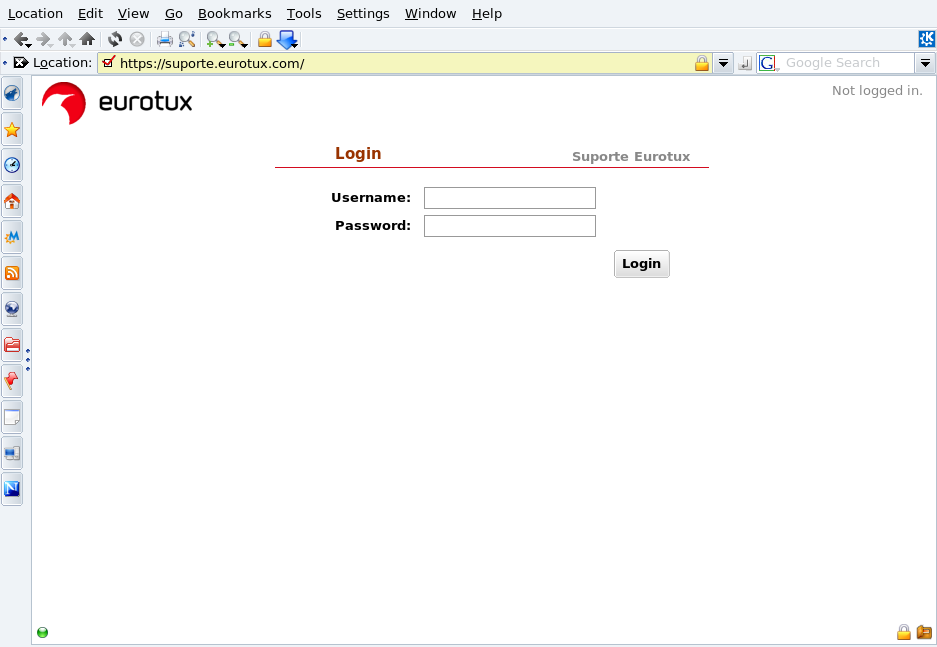
\includegraphics[scale=0.45]{include/img/rt1}
%%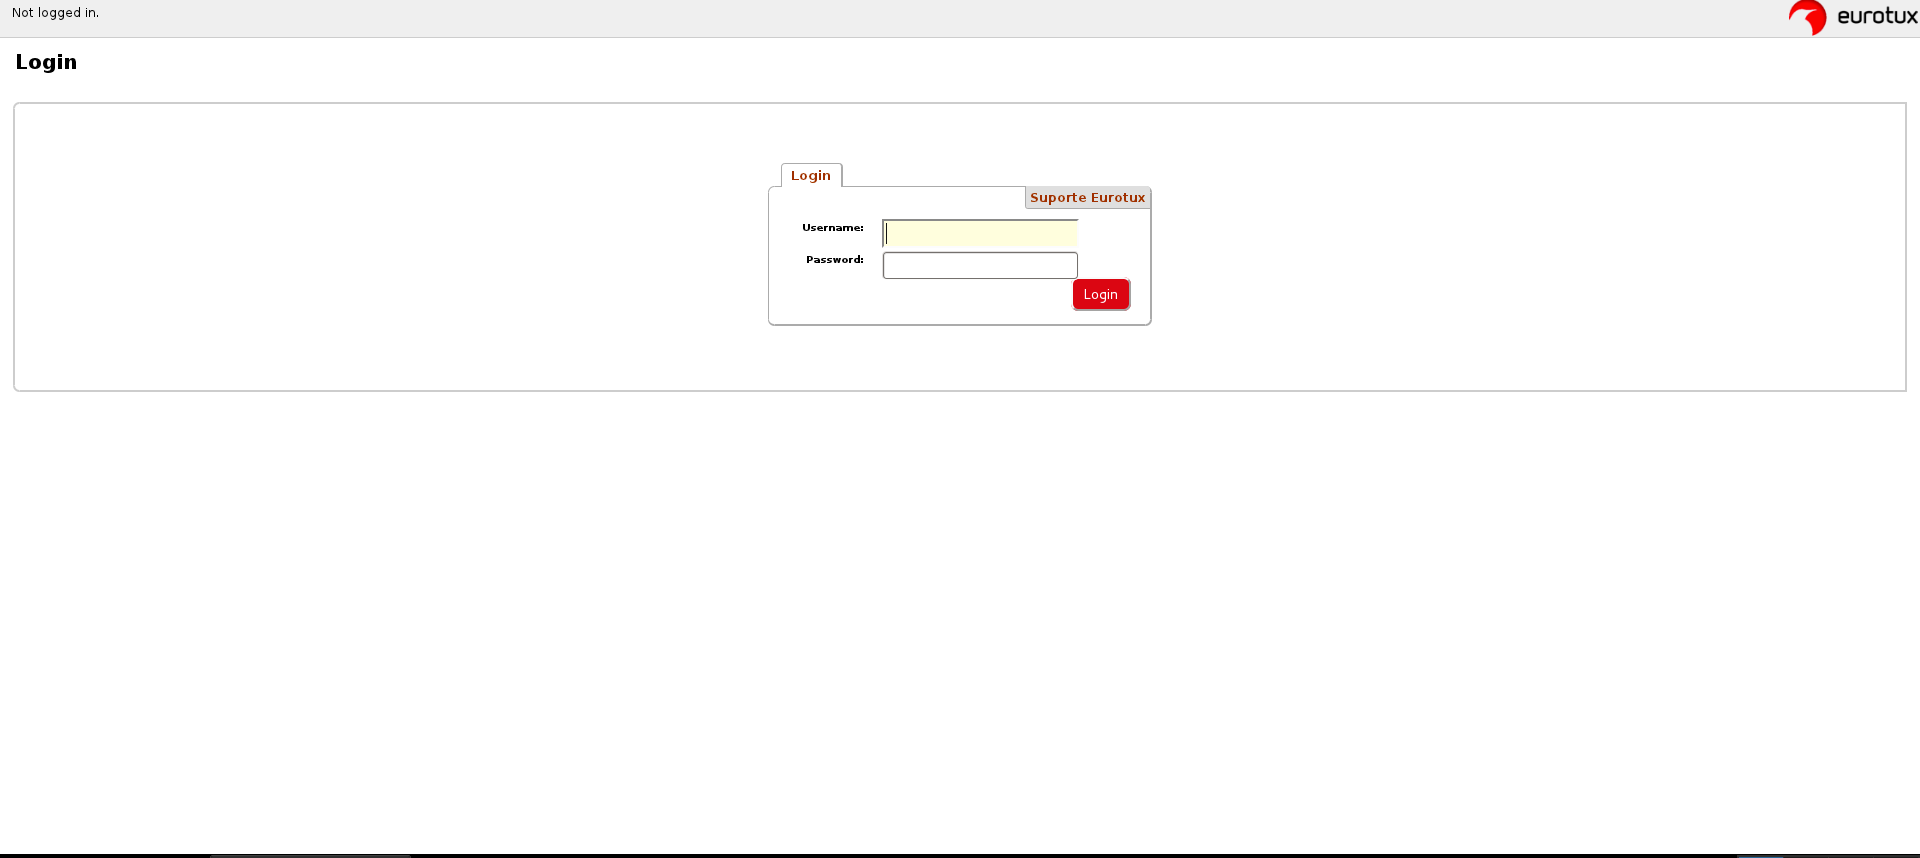
\includegraphics[width=16cm,height=10.5cm]{include/img/rt1_1}
%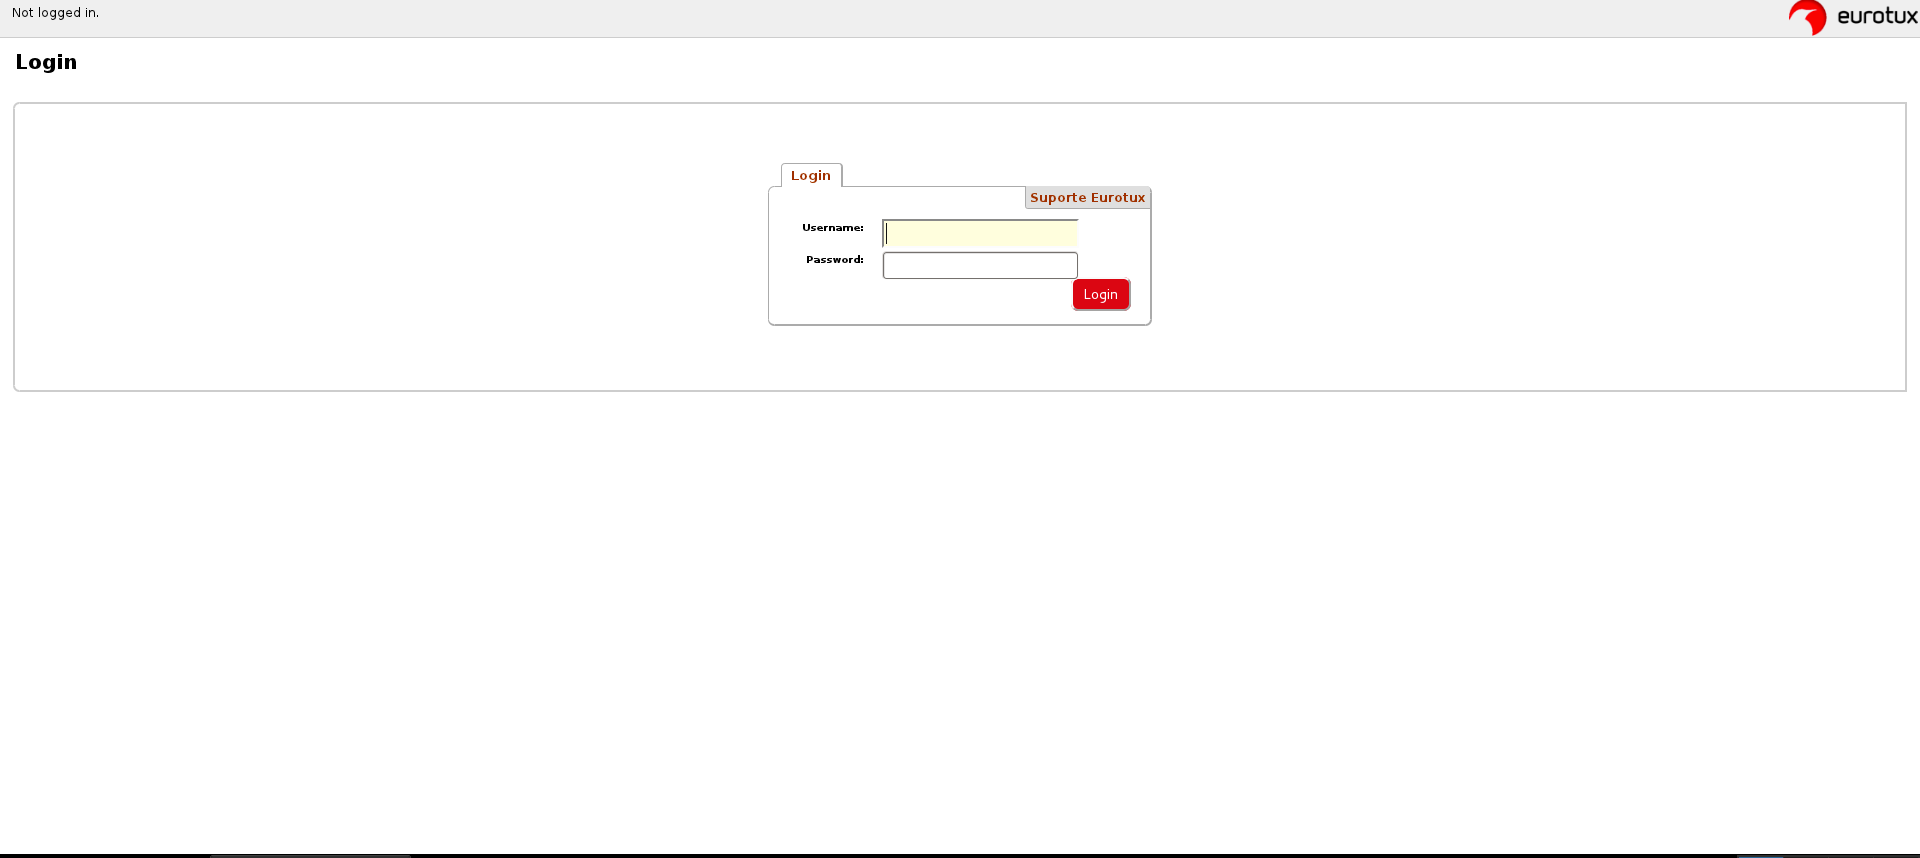
\includegraphics[width=16cm]{include/img/rt1_1}
%\end{center}
%\caption{Página de Autenticação}
%\label{fig:rt1}
%\end{figure}

\begin{figure}[H]
\begin{center}
%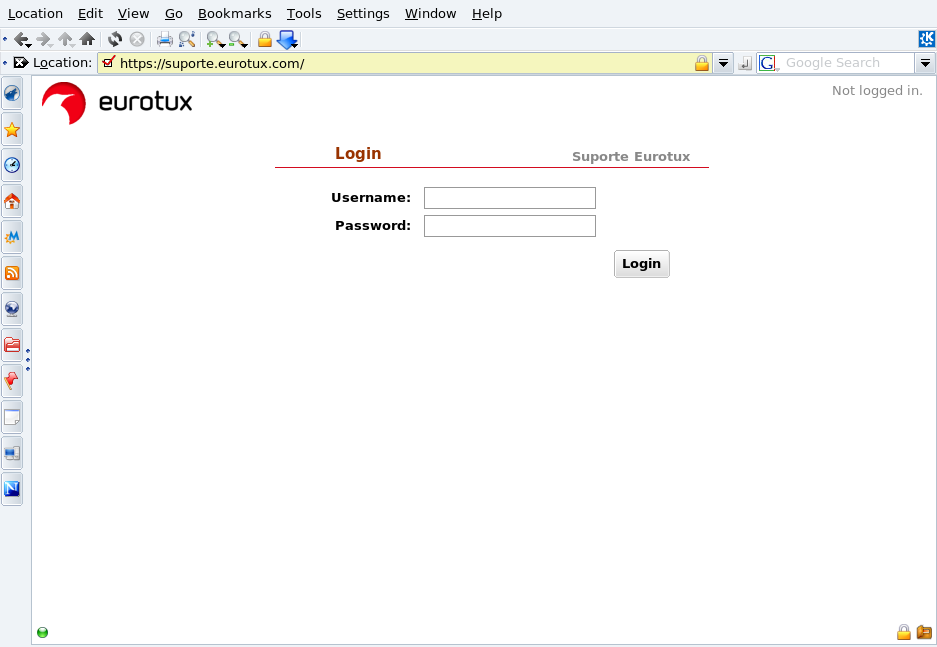
\includegraphics[scale=0.45]{include/img/rt1}
%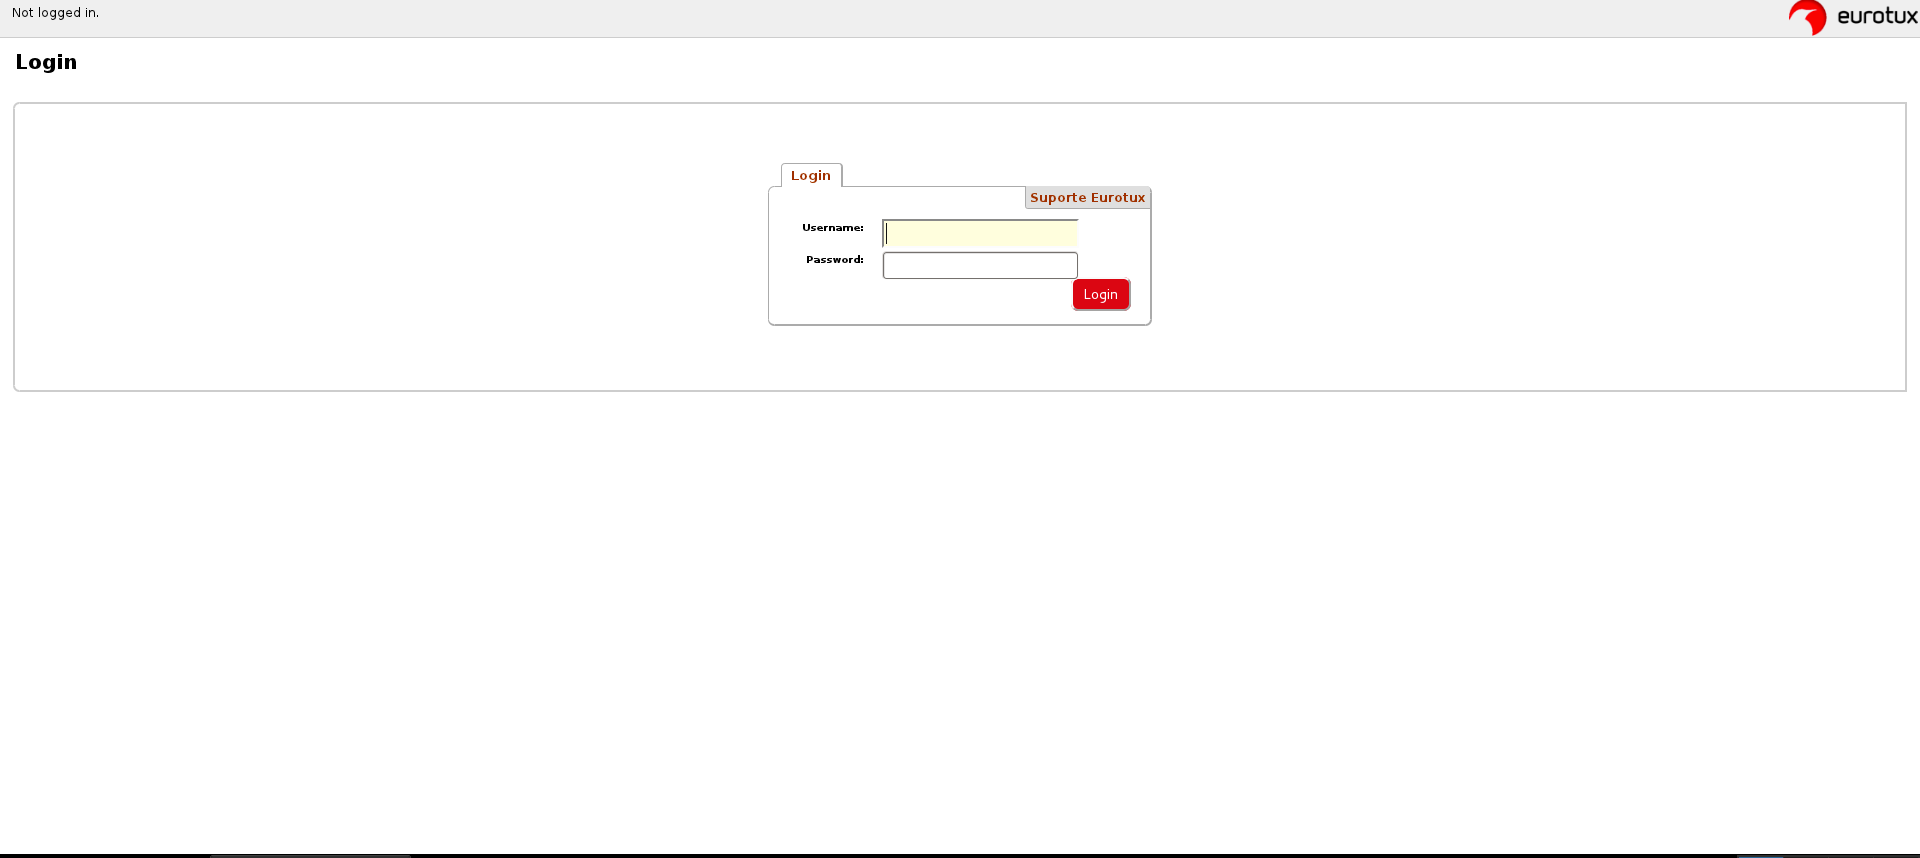
\includegraphics[width=16cm,height=10.5cm]{include/img/rt1_1}
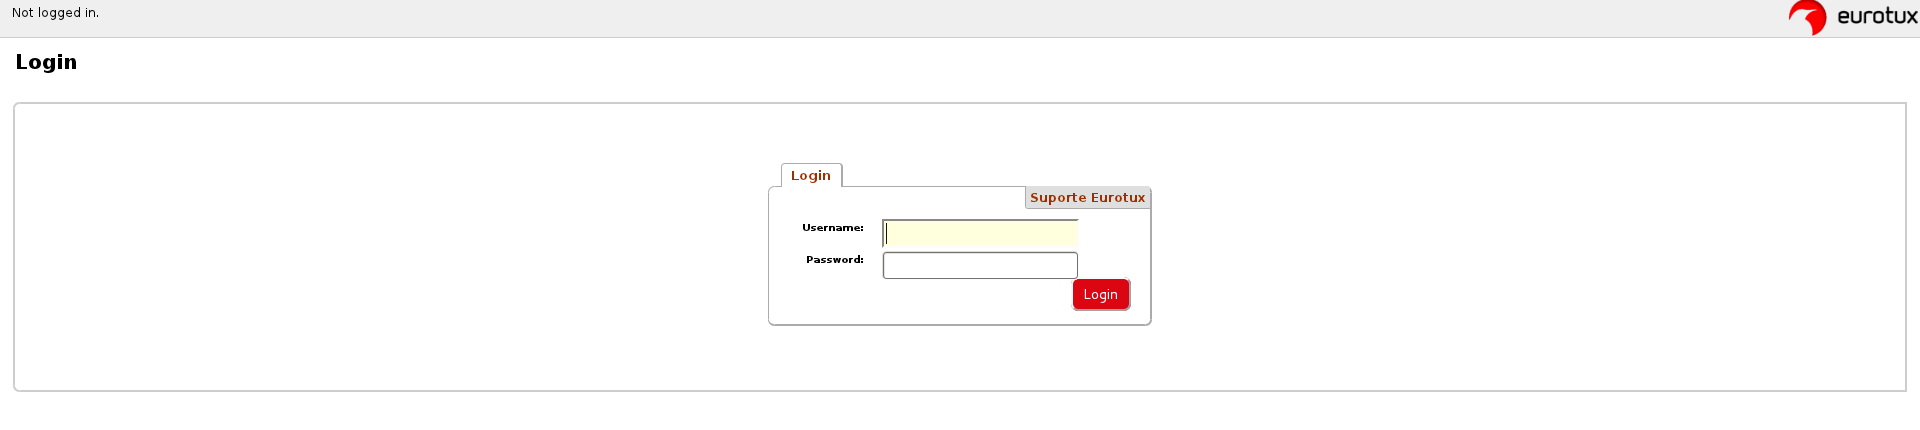
\includegraphics[width=16cm]{\directorynameimg/rt1-1}
\end{center}
\caption{Página de Autenticação}
\label{fig:rt1}
\end{figure}

\section{Página inicial}
Após efectuar o \emph{login} no SGI, será encaminhado para a página inicial (figura \ref{fig:rt2}) onde é efectuada a gestão dos pedidos de incidentes.

\begin{figure}[H]
\begin{center}
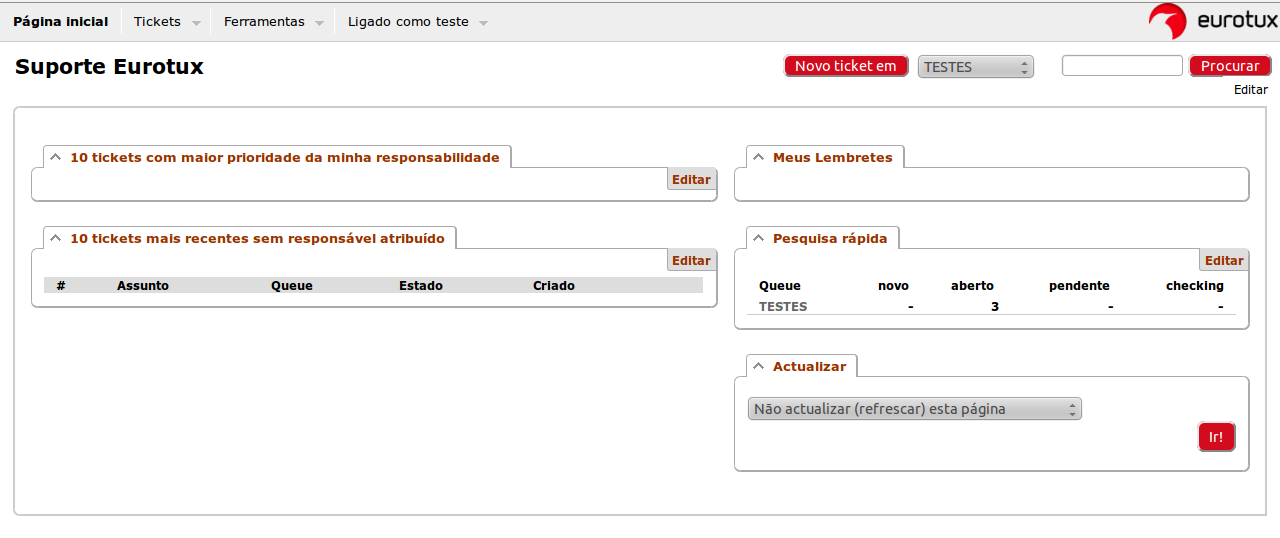
\includegraphics[width=16cm]{\directorynameimg/rt2-1-PT}
\end{center}
\caption{Página Inicial}
\label{fig:rt2}
\end{figure}

A página inicial possui vários agrupadores, que disponibilizam de uma forma organizada os pedidos de incidente que se encontram abertos.

\begin{itemize}
\item \textbf{tickets com maior prioridade da minha responsabilidade}
\subitem Neste campo são apresentados os tickets de incidentes abertos, que são da responsabilidade do utilizador.\\
É possível definir o número de tickets a visualizar neste campo e o seu modo de ordenação.

\item \textbf{tickets mais recentes sem responsável atribuído}
\subitem Neste campo são apresentados os tickets de incidentes abertos, que se encontram a aguardar pela atribuição de um técnico responsável pela resolução do incidente.\\
É possível definir o número de tickets a visualizar neste campo e o seu modo de ordenação.

\item \textbf{Meus Lembretes}
\subitem Neste campo, é possivel visualizar as notificações (ou lembretes) existentes, relativos a alguma acção associada a um ticket. Por exemplo, efectuar um contacto, fazer um ponto de situação, etc..
\item \textbf{Pesquisa rápida}
\subitem No ecrã que aparece imediatamente após o \emph{login}, existe uma coluna no lado direito identificada como \emph{Pesquisa rápida | Quick Search} em que existe um único item (\emph{queue}).
É nessa \emph{queue} que estarão os pedidos de suporte/help-desk (\emph{tickets}) ainda abertos (open).
\item \textbf{Actualizar}
\subitem Nesta caixa de selecção, é possível definir a frequência de actualização da informação disponibilizada na página inicial.
\end{itemize}


%\begin{figure}[H]
%\begin{center}
%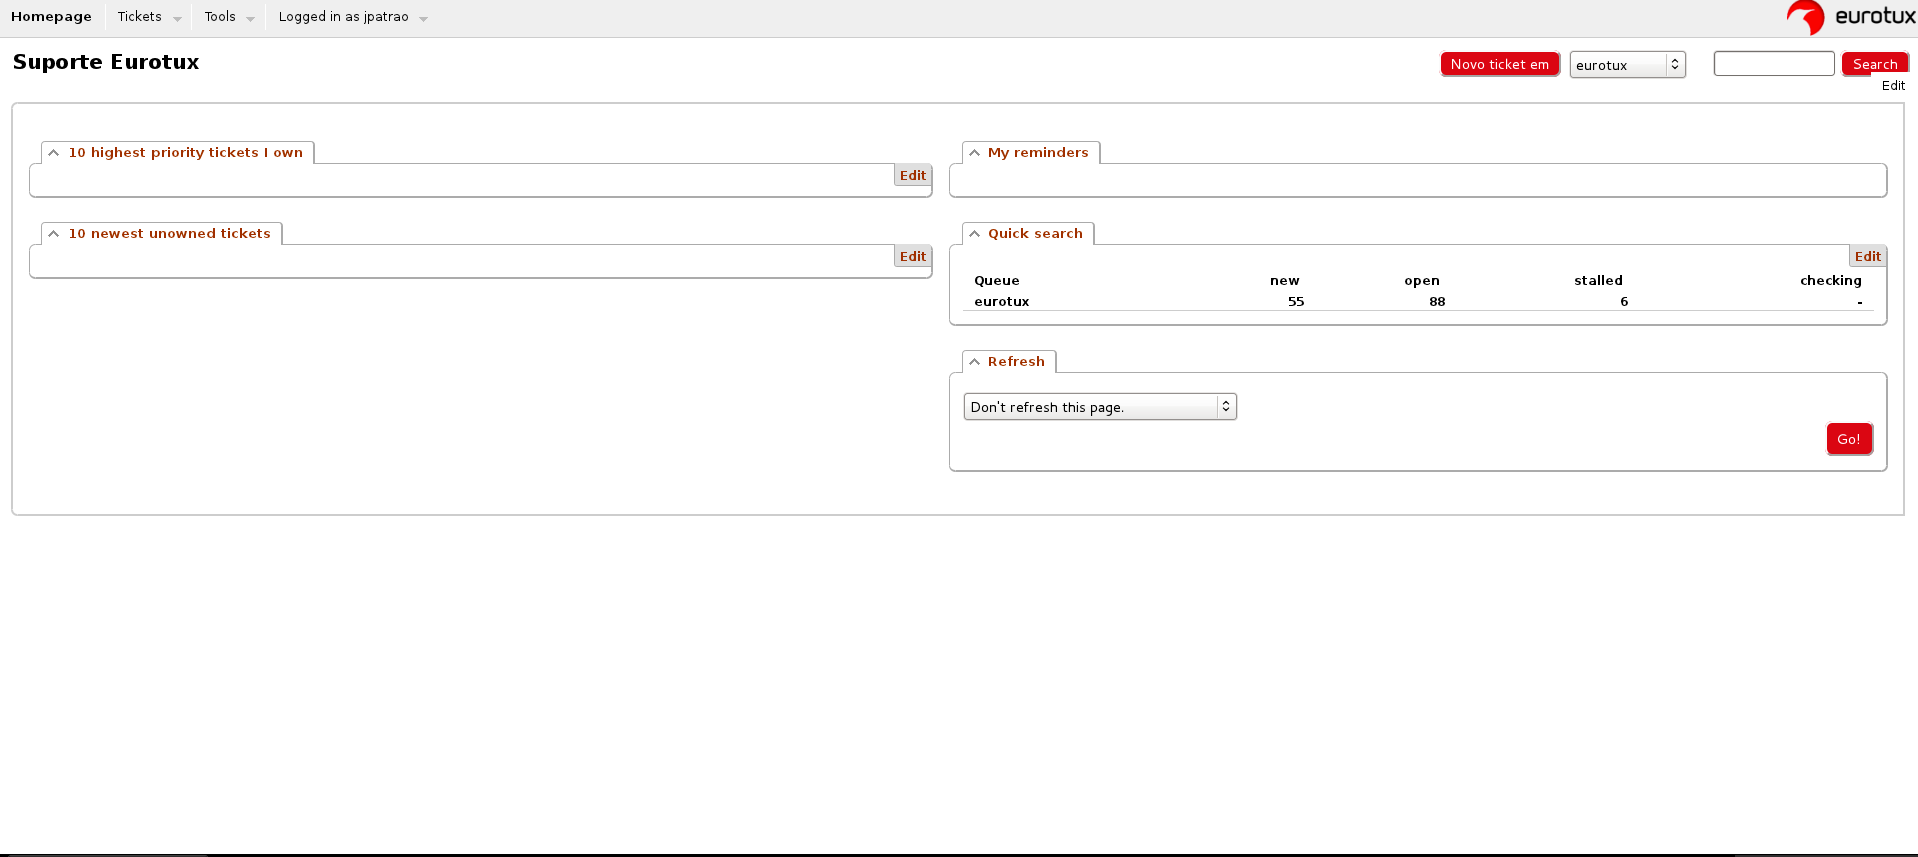
\includegraphics[width=15cm]{include/img/rt2_1}
%\end{center}
%\caption{Página Inicial}
%\label{fig:rt2}
%\end{figure}

\section{Criar \emph{Ticket}}
Para criar um novo \emph{ticket}, deverá seleccionar \emph{Novo Ticket em | New Ticket In} e depois seguir os seguintes passos:
\begin{itemize}
\item Preencher o campo \emph{Assunto | Subject}, onde será indicado o assunto relativo ao ticket;
\item Preencher o campo \emph{Descreva o pedido, abaixo | Describe the issue below} (ver figura \ref{fig:rt3}), onde deverá descrever o incidente, tentando apresentar toda a informação disponível sobre o mesmo e que possa ser de auxílio ao Departamento de Suporte na resolução do incidente;
\item Após a descrição do incidente, deverá clicar no botão \emph{Criar | Create} que se situa do lado direito, abaixo da caixa de texto da descrição do incidente;
\item Desta forma o incidente fica registado e acessível aos técnicos da Eurotux que irão aceder a informação que foi registada e à qual darão o seguimento adequado.
\end{itemize}

\bigskip

\textbf{Campos opcionais de preenchimento:}
\begin{itemize}
\item \textbf{Cc:}
\subitem Se desejar pode adicionar, neste campo, um outro endereço de email o que permitirá que as interacções no Sistema sejam enviadas para o endereço referido. Esta funcionalidade permite que um utilizador não registado na \textit{comunidade de utilizadores} \textbf{visualize} as interacções ocorridas num \emph{ticket};
\item \emph{\textbf{Anexar ficheiro | Attach file:}}
\subitem Pode anexar um ou mais ficheiros ao \emph{ticket}, para complementar a informação sobre o incidente ou para registo.
\end{itemize}

\bigskip

A \emph{comunidade de utilizadores} que acede a uma \emph{queue} recebe sempre por email o conteúdo que for colocado nessa \emph{queue} por qualquer um dos membros da \emph{comunidade de utilizadores}. A \emph{comunidade de utilizadores} é normalmente constituída pelos endereços do cliente dessa \emph{queue} (um ou mais) e pelos endereços dos técnicos da Eurotux.

Após a recepção do email mencionado no parágrafo anterior é possível responder a essa mensagem fazendo um \emph{reply} normal, escrevendo no corpo da mensagem as informações que se pretende transmitir e de imediato essa informação será adicionada ao \emph{ticket} em causa ficando imediatamente também acessível via Web (sem necessidade de aceder directamente à ferramenta). 

\textbf{NOTA}: A aplicação web só registará mensagens cujo o endereço de email coincida com um dos emails registados na \emph{comunidade de utilizadores}, o que significa se for usado qualquer outro, a mensagem não ficará registada.

Quando for efectuado reply às mensagens deve-se retirar o máximo de informação não relevante da mensagem e colocar só o que corresponde a informação nova porque a ferramenta por si já constitui um histórico das diversas interacções.


\begin{figure}[H]
\begin{center}
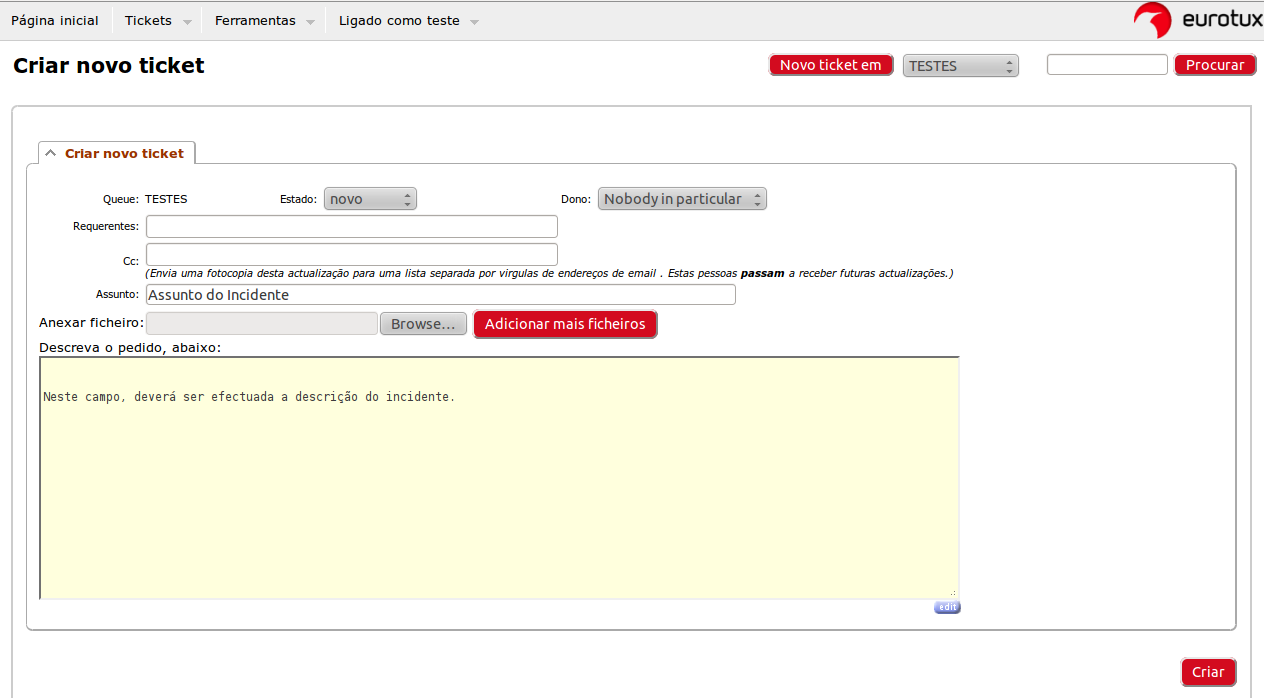
\includegraphics[width=16cm]{include/img/rt3-1-PT}
\end{center}
\caption{Criação de um \emph{Ticket}}
\label{fig:rt3}
\end{figure}

\section{Fecho de \emph{Tickets}}
Os \emph{tickets} devem ser encerrados pelo próprio cliente, constituindo o seu encerramento uma forma de aprovação e validação das actividades desenvolvidas, significando ainda que a intervenção está concluída.

Para encerrar o \emph{ticket} basta seleccionar a opção \emph{Resolver | Resolve} que aparece no menu \emph{Acções | Actions} no canto superior direito do ecrã onde se está a visualizar um determinado \emph{ticket} (ver figura \ref{fig:rt6}).

No acto de fecho de um \emph{ticket} é possível efectuar nova entrada de texto (opcional) que poderá ser, por exemplo, a confirmação de que os trabalhos foram efectuados com sucesso e o incidente se encontra resolvido, ou qualquer outra informação relevante.

Os \emph{tickets} depois de encerrados não aparecerão na visualização por omissão.

\begin{figure}[H]
\begin{center}
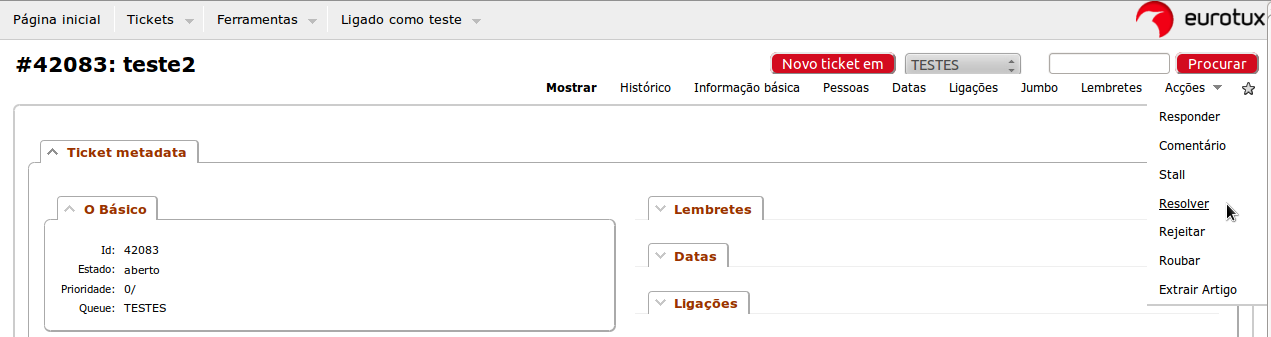
\includegraphics[width=16cm]{\directorynameimg/rt6-1-PT}
\end{center}
\caption{Fecho de ticket}
\label{fig:rt6}
\end{figure}

\section{Reclamar}
O Sistema disponibiliza uma ferramenta, denominada \emph{Reclamar}, que permite ao cliente reportar a situação quando considerar que a resposta ao incidente em questão não está a ser adequada ou satisfatória.

Para registar uma reclamação relativa a um incidente, deverá preencher o campo \emph{Reclamar} (ver figura \ref{fig:rt7}), fornecendo a descrição dos factos relevantes, e em seguida clicar no botão \textbf{enviar} que se encontra junto à caixa de texto.

A reclamação será registada e transmitida aos responsáveis do Departamento de Suporte, que efectuarão a sua análise e darão diligência aos procedimentos adequados.

\begin{figure}[H]
\begin{center}
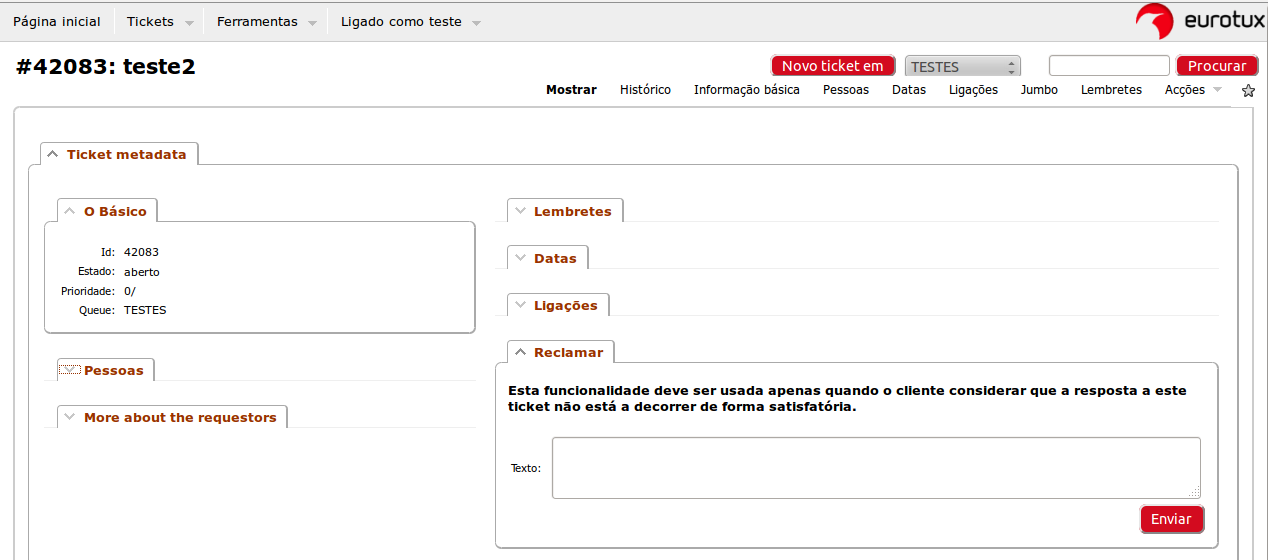
\includegraphics[width=16cm]{\directorynameimg/rt7-1-PT}
\end{center}
\caption{Fecho de ticket}
\label{fig:rt7}
\end{figure}



\section{Pesquisa de \emph{Tickets}}
O Sistema disponibiliza uma função de pesquisa de \emph{tickets}, encerrados ou abertos, permitindo fazer uma pesquisa simples (por número do ticket ou parte do texto do seu assunto) ou uma pesquisa mais avançada, podendo refinar os critérios de pesquisa.
Podem ser efectuadas pesquisas de \emph{tickets} encerrados ou ainda abertos, seleccionando no menu localizado na parte superior da página, o link \emph{Tickets}, aparecendo um menu denominado \emph{Nova Pesquisa | New Search} (ver figura \ref{fig:rt4}). De seguida deverão ser preenchidos os campos adequados para obter os \emph{tickets} que obedeçam aos critérios definidos.

Sabendo o número do \emph{ticket} é possível visualizá-lo imediatamente bastando para isso introduzir esse número na caixa que diz \emph{Search} (do lado direito, quase no topo do ecrã).

\begin{figure}[H]
\begin{center}
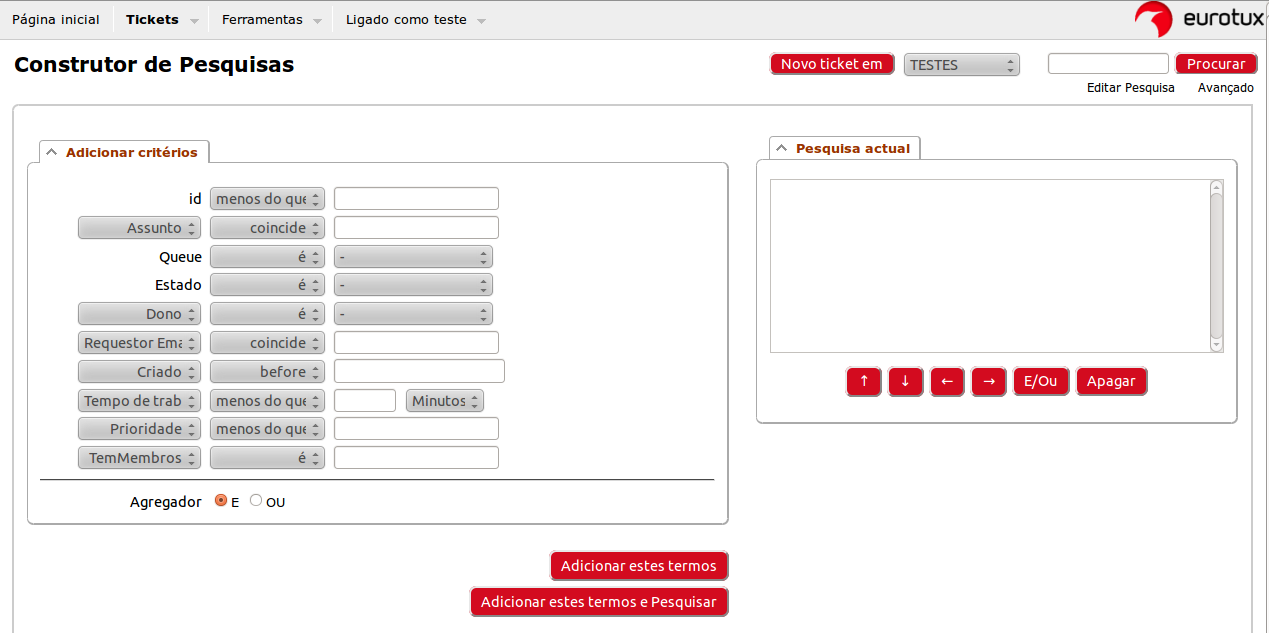
\includegraphics[width=16cm,height=9cm]{include/img/rt4-1-PT}
\end{center}
\caption{Procurar \emph{Tickets}}
\label{fig:rt4}
\end{figure}

\section{Preferências}
Uma vez dentro do Sistema de Gestão de Incidentes, recomendamos a alteração da password indicada pelo Departamento de Suporte para uma personalizada pelo utilizador.

Para alterar a sua password, deverá seleccionar o menu, \emph{Ligado como... | Logged in as...} onde aparece uma opção denominada \emph{Configurações | Settings} e escolher a opção \emph{Acerca | About} (ver figura \ref{fig:boot}). Neste painel pode ser alterada a password de acesso à ferramenta web, o idioma e outros dados acerca do utilizador.

Também recomendamos que, na selecção do idioma para Português, seja utilizado a opção \textbf{Portuguese} em vez das opções Portuguese (Portugal) ou Portuguese (Brazillian).

\begin{figure}[H]
\begin{center}
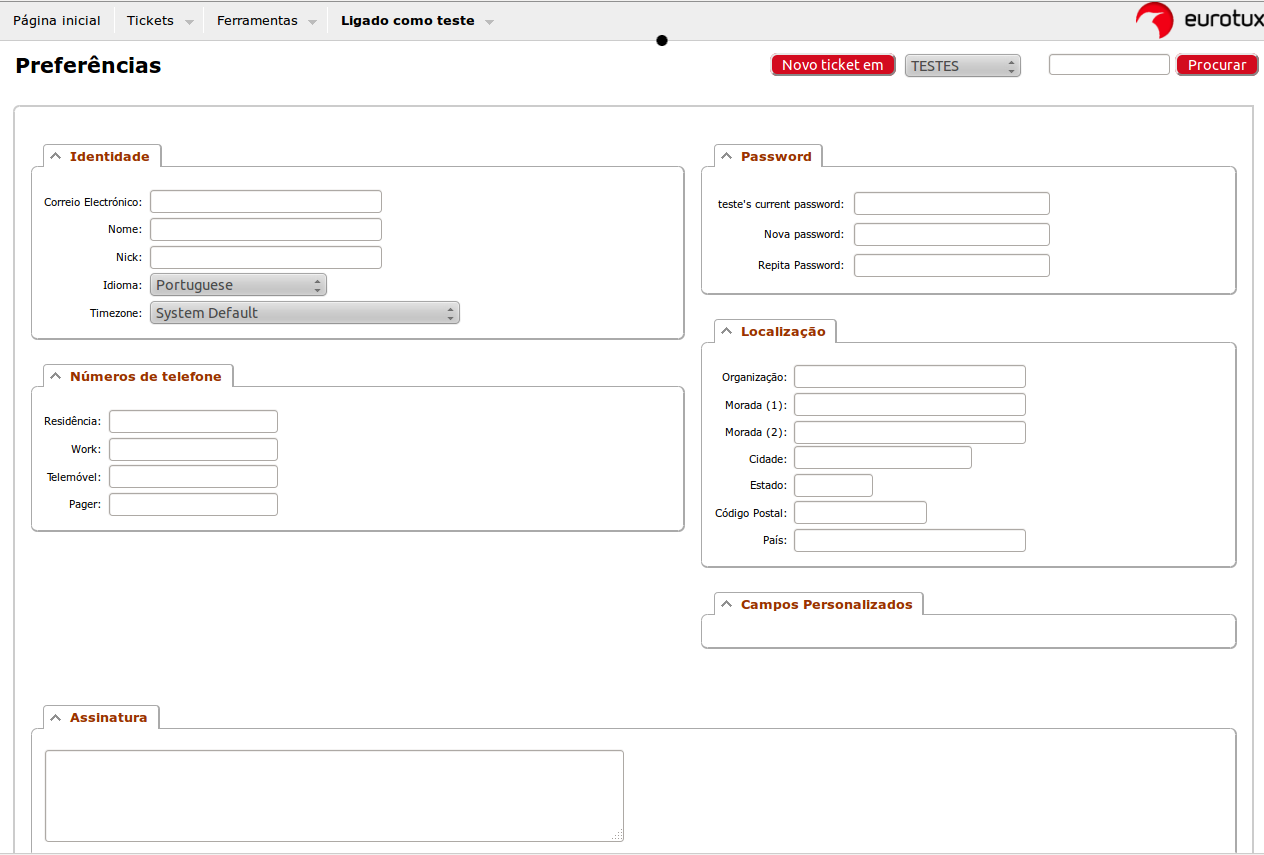
\includegraphics[width=16cm,height=10.5cm]{include/img/rt5-1-PT}
\end{center}
\caption{Alterar Preferências}
\label{fig:boot}
\end{figure}

\section{Sair}
Esta opção efectua o \textit{logout} do utilizador, encerrando a sessão e sendo encaminhado para a página inicial, onde poderá efectuar \textit{login} novamente, se o desejar.



%\chapter{Página Inicial}
%\section{Descrição}
%
%\chapter{Tickets}
%\section{Descrição}
%\section{Pesquisa Simples}
%\section{Nova Pesquisa}
%
%\chapter{Ferramentas}
%\section{Descrição}
%\section{Artigos}
%\subsection{Visão Geral}
%\subsection{Procura}
%\subsection{topics}
%\section{O Meu Dia}
%\section{Meus Lembretes}
%\section{Offline}
%\section{Aprovação}
%
%\chapter{Ligado como ...}
%\section{Descrição}
%Nesta aba é disponibilizado o acesso às opções de configuração do sistema e a opção para o utilizador efectuar o \textit{logout} do sistema.
%\section{Configurações}
%\subsection{Opções}
%\subsection{Acerca}
%\subsection{Opções de Pesquisa}
%\subsection{Vista inicial RT}
%\subsection{Pesquisa Rápida}
%\subsection{Pesquisas Guardadas}
%\subsubsection*{My Tickets}
%\subsubsection*{Unowned Tickets}
%\subsubsection*{Bookmarked Tickets}
%\section{Sair}
